%\documentclass[useAMS, usenatbib,usegraphicx,letter]{mn2e}
%\documentclass[11pt]{article}
\documentclass[reprint,aps,prd,superscriptaddress,showkeys,showpacs]{revtex4-1}
\usepackage{epsfig,amsmath,natbib}

\usepackage{aas_macros}
\usepackage{amssymb}
\usepackage{amsmath}
\usepackage{dsfont}
\usepackage{hyperref}
\usepackage{color}
\usepackage{pbox}
\usepackage{booktabs}
\usepackage[dvipsnames]{xcolor}

\hypersetup{
	colorlinks=false,
	citecolor=green
}
% \usepackage{graphicx}
% \usepackage{epstopdf}
% \usepackage{natbib}

%%%%%%%%%%%%%%%%%
%Custom commands%
%%%%%%%%%%%%%%%%%

\newcommand{\bb}[1]{\mathbf{#1}}
\newcommand{\bbh}[1]{\mathbf{\hat{#1}}}
\newcommand{\h}[1]{\hat{#1}}

%%%%%%%%%%%%%%%%%%%%%%%%%%%%%%%%%%%%%%%%%%%%%%

\begin{document}

\title{Simulating cosmic variance in Weak Lensing: effects on parameter inferences}

\author{Andrea Petri}
\email{apetri@phys.columbia.edu}
\affiliation{Department of Physics, Columbia University, New York, NY 10027, USA}
\affiliation{Physics Department, Brookhaven National Laboratory, Upton, NY 11973, USA}

\author{Zolt\'an Haiman}
\affiliation{Department of Astronomy, Columbia University, New York, NY 10027, USA}

\author{Morgan May}
\affiliation{Physics Department, Brookhaven National Laboratory, Upton, NY 11973, USA}

\date{\today}

\label{firstpage}

\begin{abstract}
Constraining cosmology using Weak Gravitational Lensing consists in comparing measured features with simulated ones. An accurate estimate of the feature covariance matrix is essential to obtain accurate parameter confidence intervals. When this covariance matrix $\bb{C}$ is measured from simulations, an important question to ask is how big the simulation set should be for an accurate estimation of $\bb{C}$. We construct different mock ensembles with $N_r$ realizations of the same shear field, based on $N_s<N_r$ independent $N$--body simulations. Using the shear--shear power spectrum as a summary statistic, we find that a single $N$--body simulation can be recycled a large number of times to produce an ensemble of $N_r=10^5$ shear realizations that are mutually independent. We also find that, for a range of summary statistics that include shear--shear power spectra measured at different scales and convergence peak counts, parameter constraints degrade faster than the $O(N_b)$ prediction by \citep{DodelsonSchneider13}, where $N_b$ is the length of the feature vector.       
\end{abstract}


\keywords{Weak Gravitational Lensing --- Simulations --- Methods: numerical,statistical}
\pacs{98.80.-k, 95.36.+x, 95.30.Sf, 98.62.Sb}

\maketitle


%%%%%%%%%%%%%%%%%%%%%%%%%% INTRO %%%%%%%%%%%%%%%%%%%%%%%%%%%%%%%%%%%%%%%%%%%%%%%%%%%%%%%%

\section{Introduction}
%
Weak Gravitational lensing is a promising cosmological probe for constraining the Dark Energy equation of state $w$, and has been considered by a range of past (CFHTLens \citep{cfht1,cfht2}), current (DES \citep{DES}) and future (LSST \citep{LSST}) experiments. In an era where cosmology is becoming data driven, accurate numerical simulations of shear fields are becoming important for a number of reasons including the study of baryonic effects \citep{BaryonXiuyuan}, non--Gaussian statistics \citep{PeaksJan,MinkJan,MinkPetri} and various systematics. Building cosmological predictions from simulations naturally introduces fluctuations in the forecasts, mainly due to cosmic variance. These fluctuations have been shown to have non negligible effects on estimates of features covariance matrices and hence on parameter constraints (see \citep{DodelsonSchneider13}). This work studies this issue further, focusing on the number of independent $N$--body simulations that is necessary to run for obtaining accurate estimates of parameter constraints, with particular focus on $w$. This paper is organized as follows: in the first paragraph we briefly describe the shear simulation methods we used, as well as the formalism we adopted to compute cosmological parameter constraints. We then outline our main findings and discuss the results, as well as future prospects for continuing this study.  

%%%%%%%%%%%%%%%%%%% METHODS %%%%%%%%%%%%%%%%%%%%%%%%%%%%%%%%%%%%%%%

\section{Methods}

\subsection{Shear field simulations}
\label{shearsim}
%
In this paragraph we describe how we constructed our shear field ensembles. Background galaxies at redshift $z_s$ are lensed by large scale structure between $z=0$ and $z_s$. The shape distortions due to the cosmic shear $\pmb{\gamma}$ can be computed in terms of the dark matter gravitational potential $\Phi(\bb{x},z)$. Because the evolution of $\Phi$ in redshift is non--linear, its evolution needs to be computed with numerical simulations. We make use of the public code \texttt{Gadget2} \citep{Gadget2}, with which we run a sequence of dark--matter--only $N$--body simulations that track the evolution of the density fluctuations in the large scale structure of the universe. We assume a standard $\Lambda$CDM framework with $(\Omega_m,\Omega_\Lambda,h,w,\sigma_8,n_s)=(0.26,0.74,0.72,-1,0.8,0.96)$ and we fix the comoving size of the simulation box to $240\mathrm{Mpc}/h$. We fill the box with $512^3$ particles, which correspond to a mass resolution of $10^{10}M_\odot$. We assume a uniform galaxy distribution at a constant redshift $z_s=2$ (at which the simulation box has an angular size of $\theta_{box}=3.5\mathrm{deg}$) and we disctretize the mass distribution between $z_s$ and the observer at $z=0$ with a sequence of 46 two dimensional lenses of thickness $80\mathrm{Mpc}/h$. The surface density on each lens is computed by projecting the three dimensional density measured from \texttt{Gadget2} snapshots. We then apply the multi--lens--plane algorithm (see \citep{RayTracingHartlap,RayTracingJain} for example) to trace the deflections of $2048^2$ light rays arranged on a square grid of total size $\theta_{box}$, from $z=0$ to $z_s$. The light deflection calculations have been performed with our implementation of multi--lens--plane algorithm, which is part of the \texttt{LensTools} computing package \citep{LensTools} (released under the \texttt{MIT} license). Different realizations $r$ of the same shear field $\pmb{\gamma}_r(\pmb{\theta})$ can be generated with different choices of the lenses that lay between the observer and $z_s$. The randomization procedure we adopt is the following:

\begin{itemize}
\item Pick a lens redshift $z_l$, and select the snapshot at $z_l$ from the $i$--th $N$--body simulation at disposal, where $i$ is a random number in $[1,N_s]$
\item Choose randomly a direction in $(\bb{n}_x,\bb{n}_y,\bb{n}_z)$: the lens plane will be pependicular to this direction
\item Choose the cutting point of the plane in the snapshot: because the lenses are $80\mathrm{Mpc}/h=240/3\mathrm{Mpc}/h$ thick, we have 3 different possibilities for choosing the random cut point
\item Perform a periodical random shift of the lens plane along its two directions
\item Repeat this procedure for each lens redshift $z_l$  
\end{itemize}  
%
This randomization procedure allows us to produce an arbitrary number $N_r$ of mock shear realizations $\pmb{\gamma}_r(\pmb{\theta})$, which however will not be all independent if $N_s$ is not large enough. Using a set of 200 independent $N$--body simulations, we construct different ensembles with different choices of $N_s\in[1,200]$, each made of 1000 mock shear realizations. We also build an additional ensemble with $N_s=1$ and $10^5$ mocks. From each of these mocks we reconstruct the convergence $\kappa_r(\pmb{\theta})$ and measure its angular power spectrum $P^{\kappa\kappa}_r(l)$ defined as
\begin{equation}
\langle\tilde{\kappa}_r(\bb{l})\tilde{\kappa}_r(\bb{l}')\rangle = (2\pi)^2\delta_D(\bb{l}+\bb{l}')P^{\kappa\kappa}_r(l)
\end{equation}
%
As an additional summary statistic, we consider the counts of local $\kappa$ maxima of a certain height $\kappa_0$, $n_r(\kappa_0)$ (from now on \textit{peak counts}), with varying $\kappa_0$. The fact that the ensemble of $N_r$ mocks is not completely independent if $N_s$ is not large enough can have an effect on the covariance estimators of $P^{\kappa\kappa},n(\kappa_0)$. 

%%%%%%%%%%%%%%%%%%%%%%%%%%%%%%%%%%%%%%%%%%%%%%%%%%%%%%%%%%%%%%%%%%%%%%

\begin{figure*}
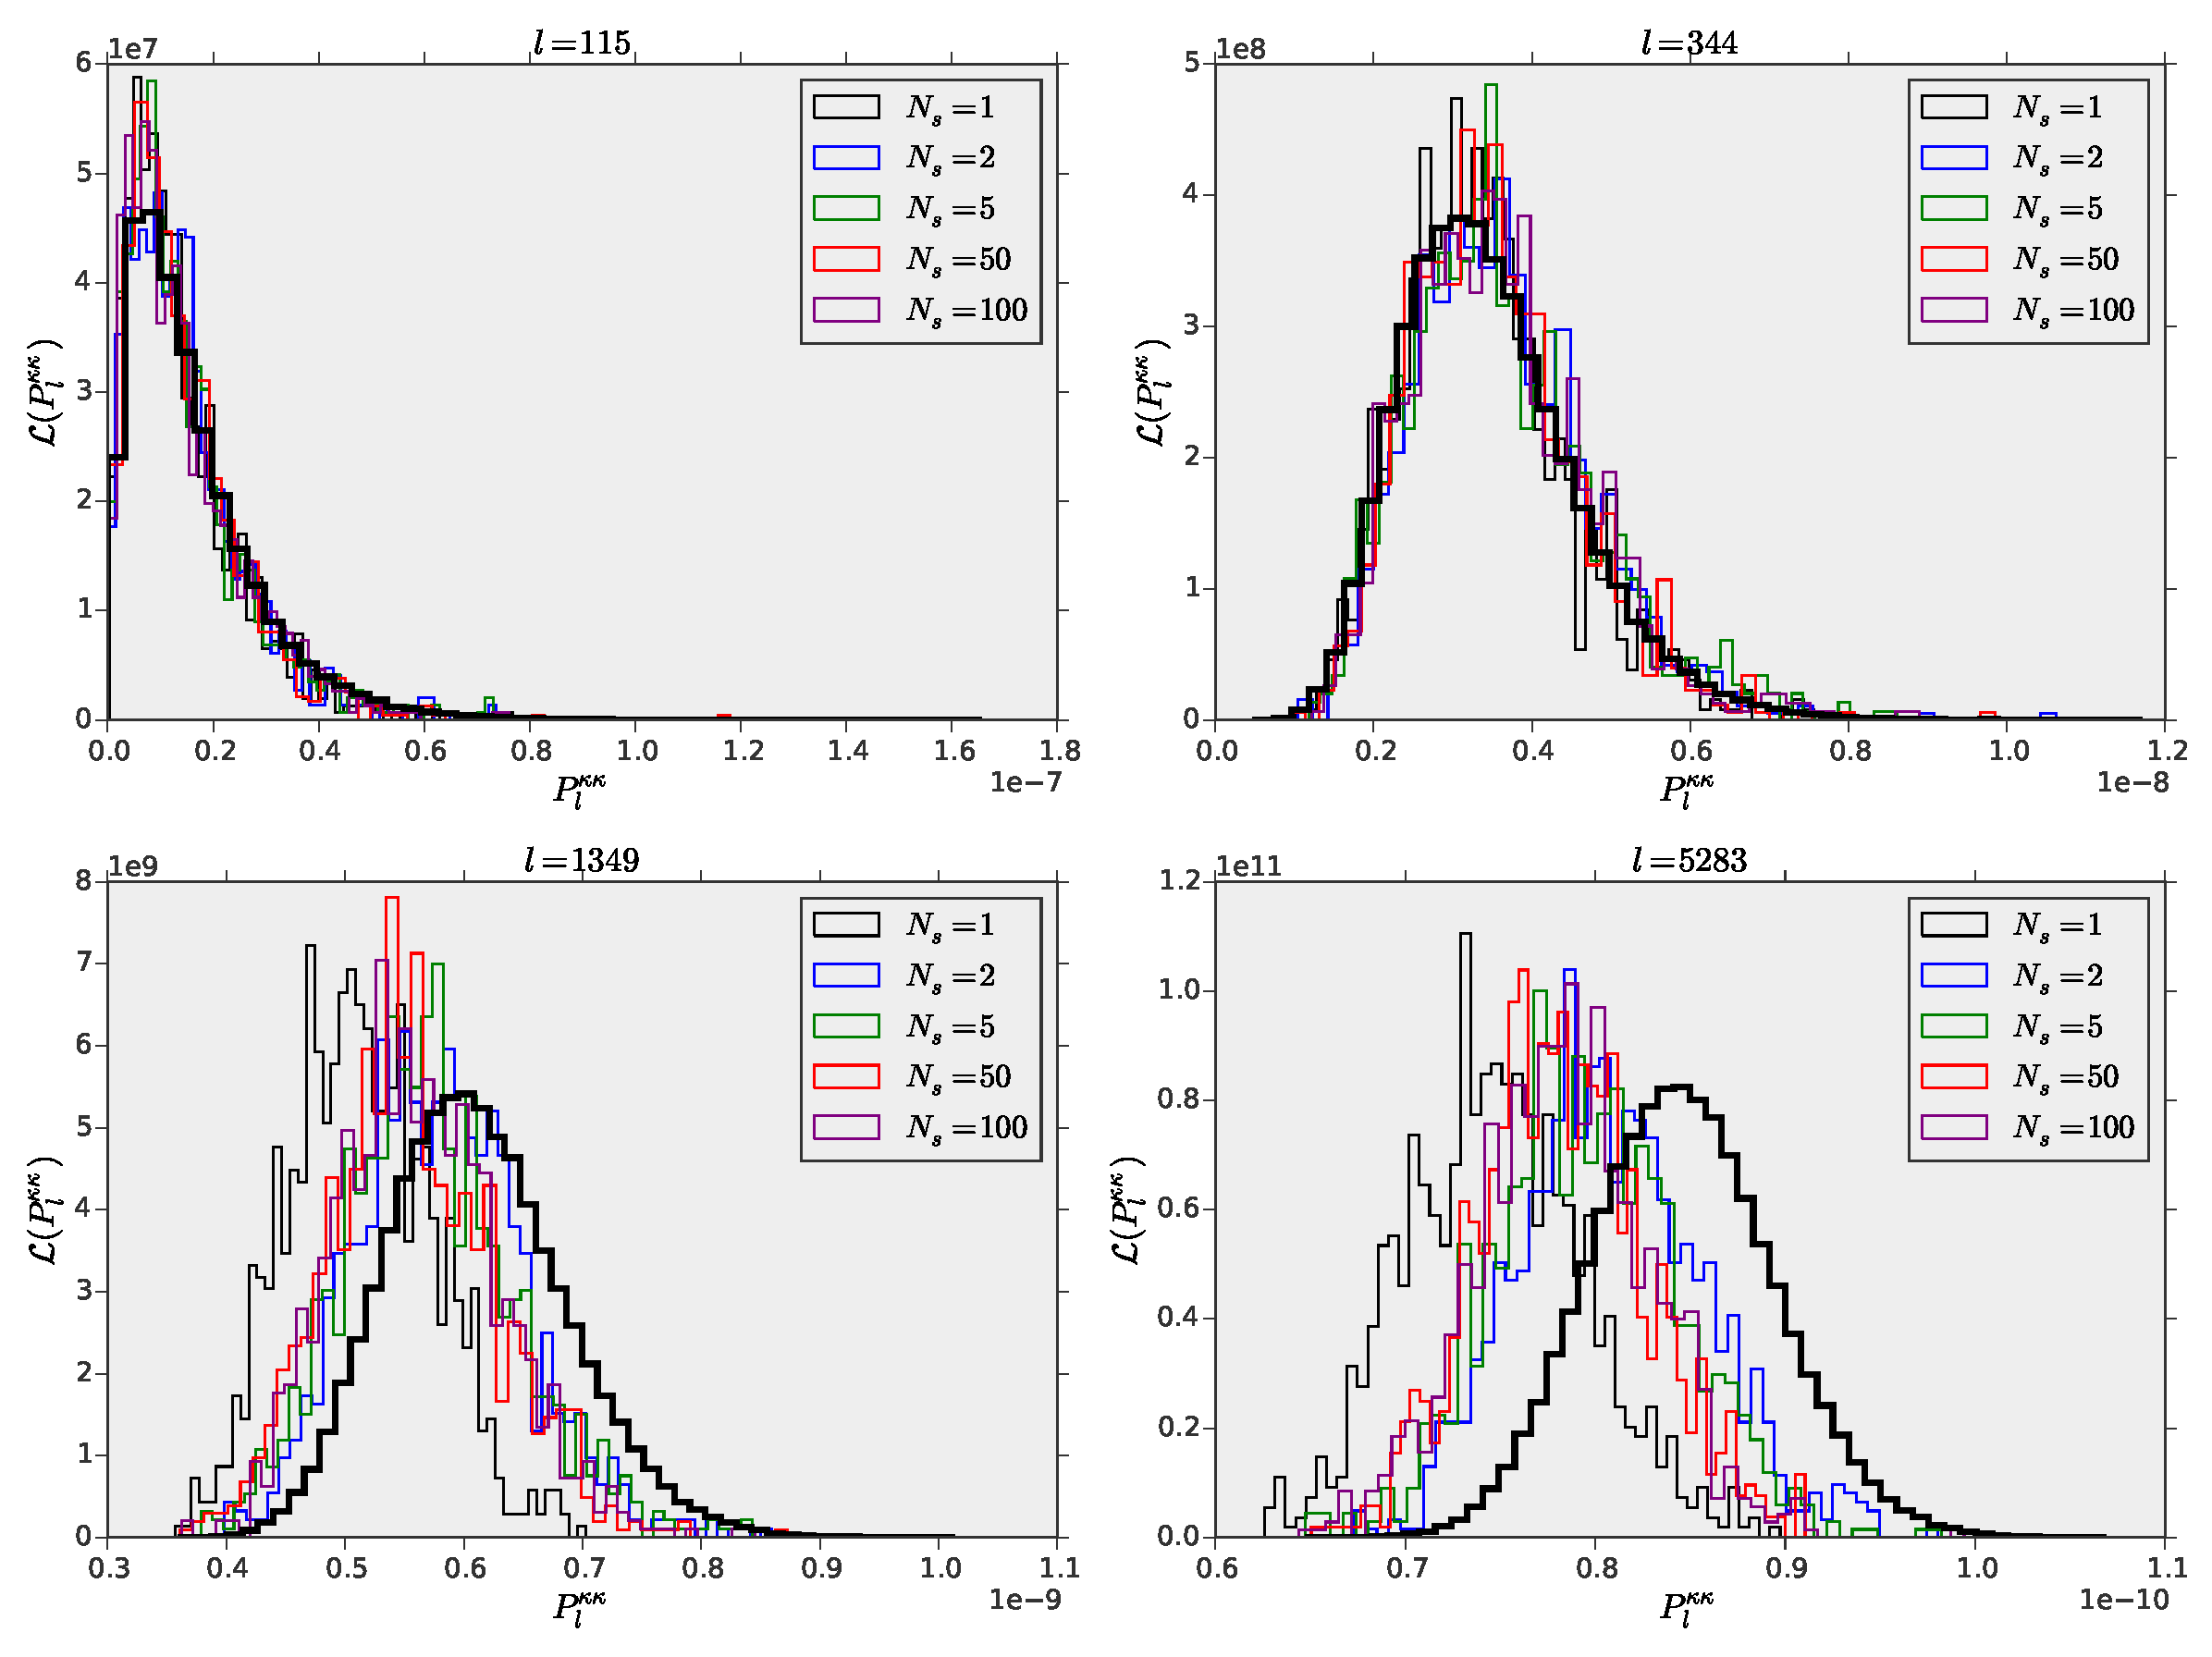
\includegraphics[scale=0.4]{Figures/ps_pdf.eps}
\caption{PDF of the $\kappa$ power spectrum,$\mathcal{L}(P_l^{\kappa\kappa})$, at four selected multipoles $l=115,344,1349,5283$, for different shear ensembles constructed with $N_s=$1 (black), 2 (blue), 5 (green), 50 (red), 100 (purple). The thick black lines correspond to an ensemble generated with $N_s=1$ and $10^5$ mock realizations.}
\label{ps_pdf}
\end{figure*}

\begin{figure}
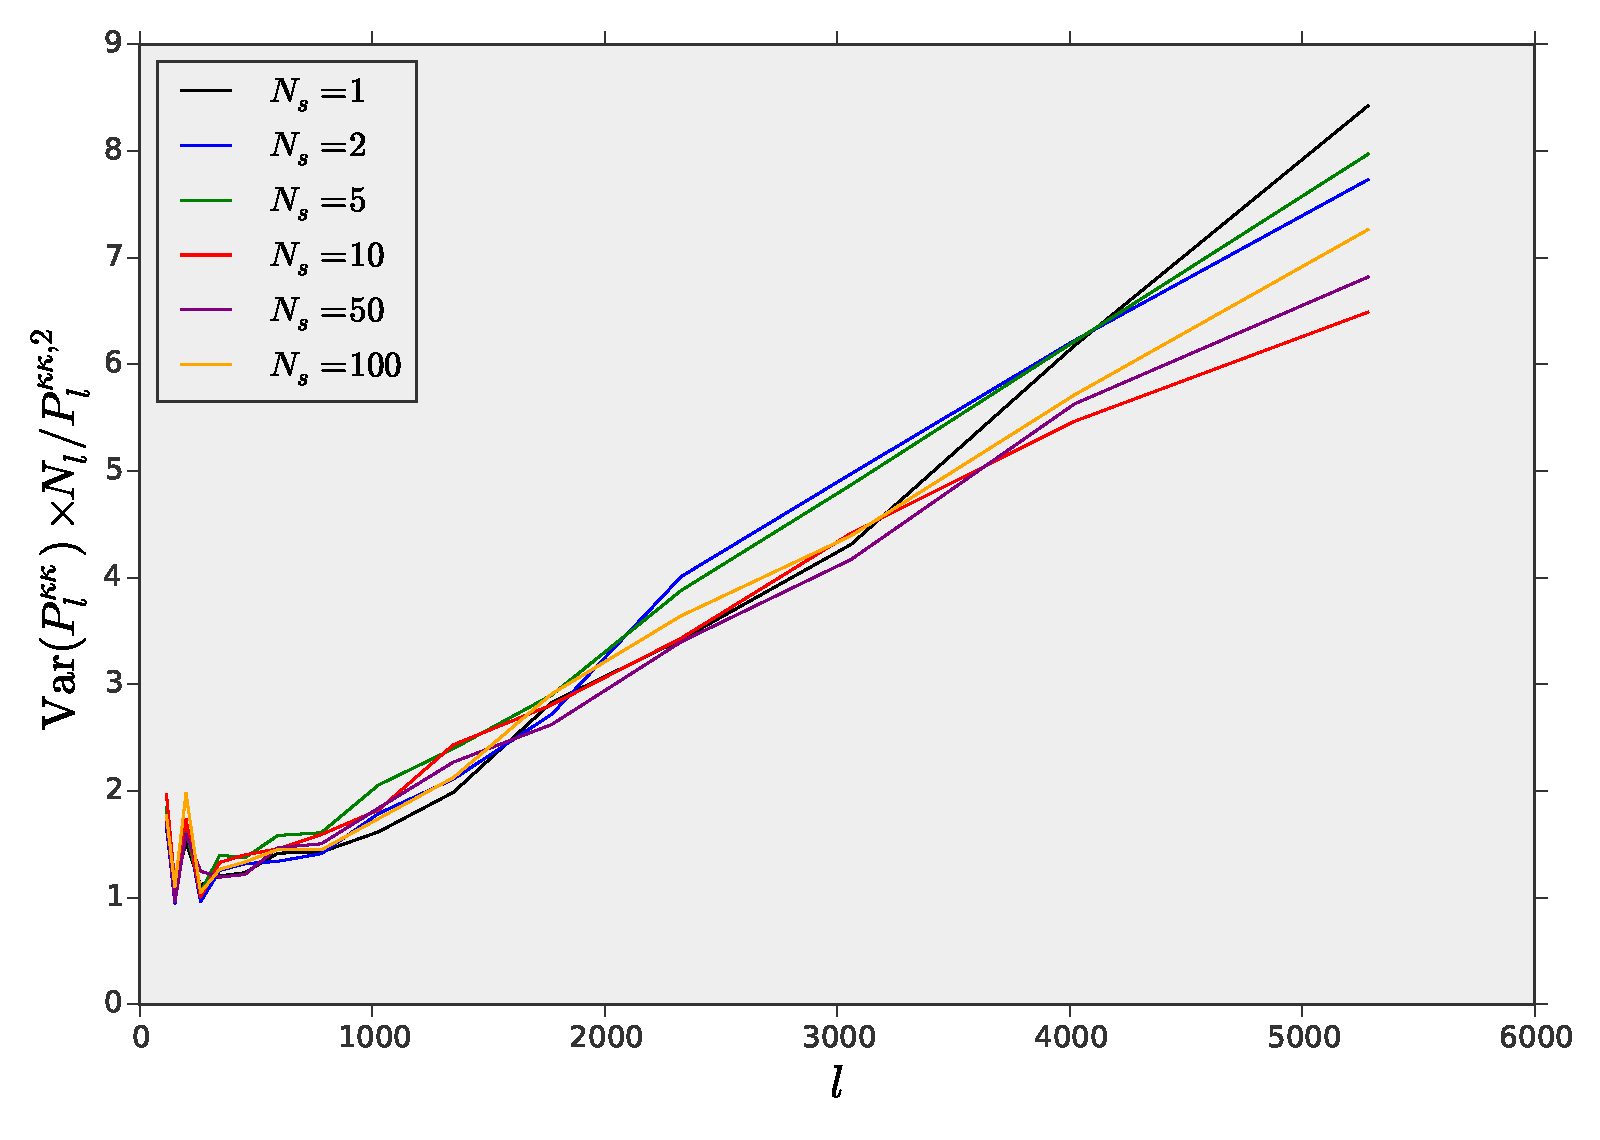
\includegraphics[scale=0.3]{Figures/ps_variance.eps}
\caption{Variance of the $\kappa$ power spectrum as a function of the multipole $l$, in units of the expected gaussian variance from equation (\ref{gaussianvar}). The variance is measured from different shear ensembles with $N_s=$1 (black), 2 (blue), 5 (green), 10 (red), 50 (purple), 100 (orange). }
\label{ps_var}
\end{figure}

\begin{figure}
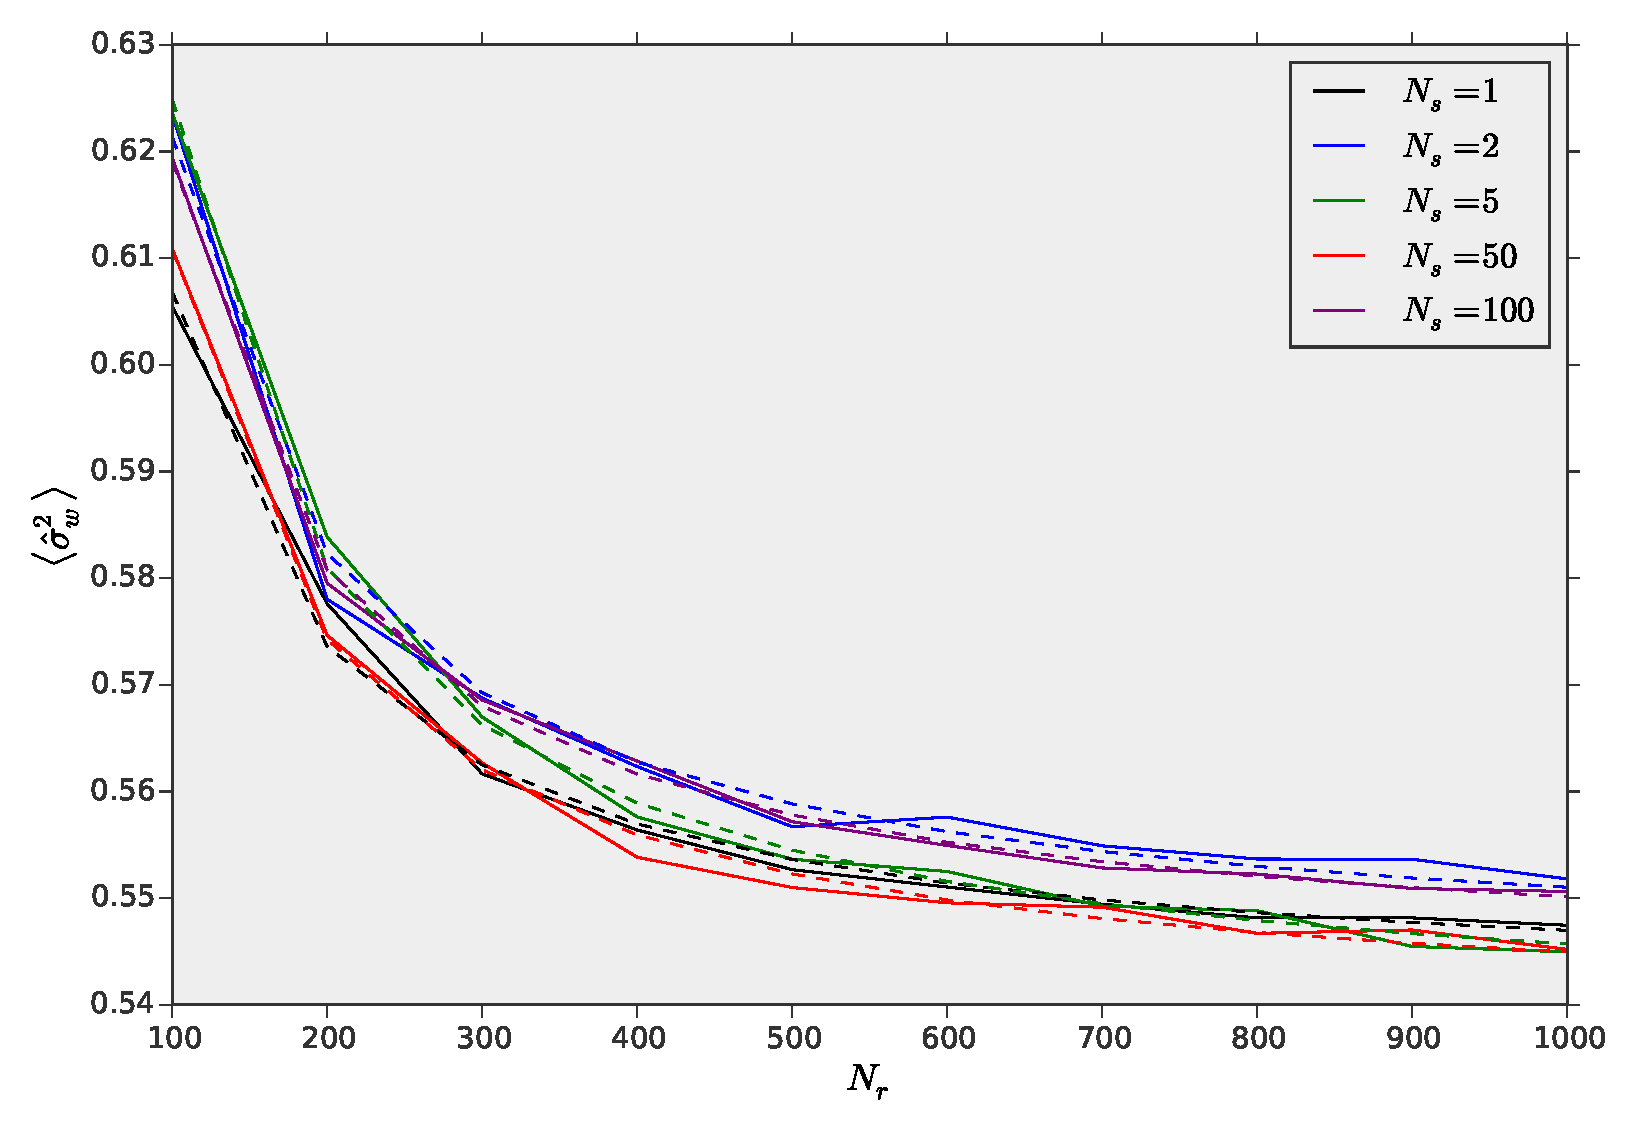
\includegraphics[scale=0.3]{Figures/scaling_nr.eps}
\caption{Bias in the $w$ variance, $\langle\h{\sigma}^2_w\rangle$, as a function of the number of mock realizations $N_r$ used in the feature covariance estimator (\ref{covest}). Results for different mock ensembles generated with $N_s=$1 (black), 2 (blue), 5 (green), 50 (red), 100 (purple) are shown. The figure shows both the measured trends (solid lines) and their best fits according to equation (\ref{ourscaling}). The thick black line correspond to an ensemble generated with $N_s=1$ and $10^5$ mock realizations. }
\label{wvar_nr}
\end{figure}

\begin{figure}
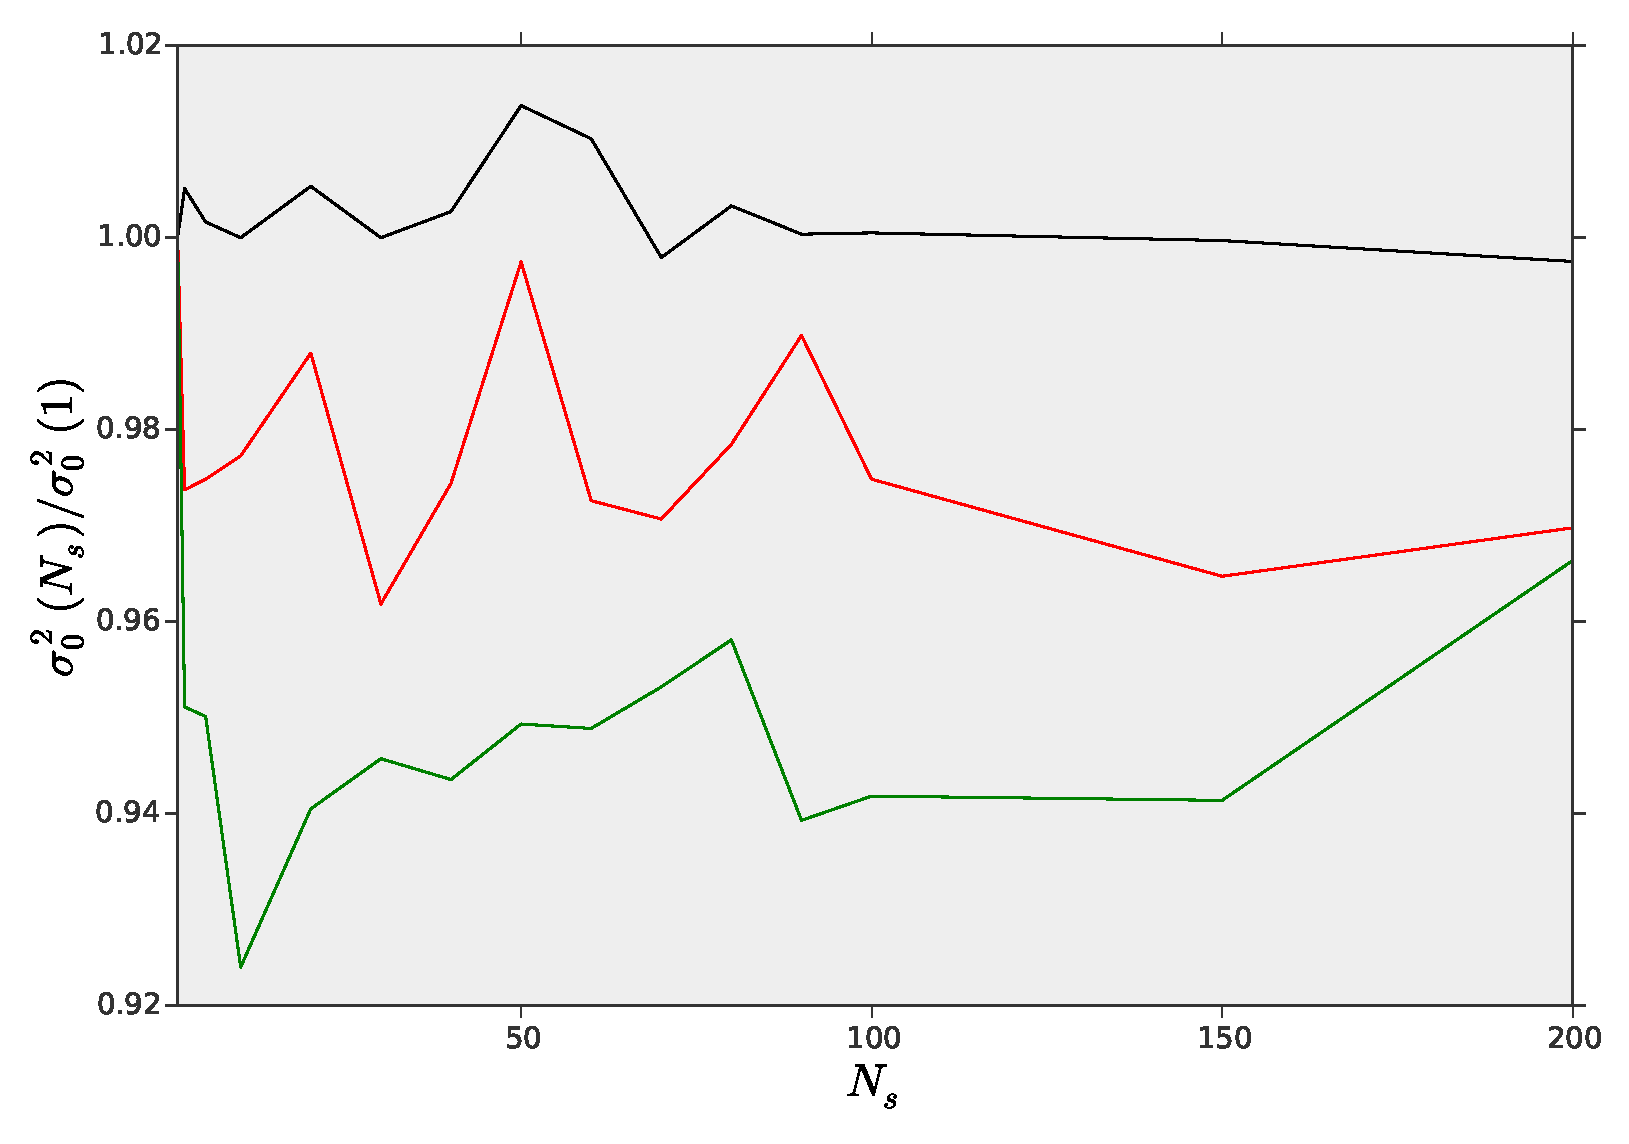
\includegraphics[scale=0.3]{Figures/scaling_ns.eps}
\caption{Variance on $w$ in the limit $N_r\rightarrow\infty$, varying the mock ensemble used to compute the covariance estimator (\ref{covest}). We show the dependence of $\sigma_0^2(N_s)$ in units of the mean over $N_s$, for the power spectrum logarithmically binned (black), the power spectrum linearly binned (red) and the peak counts (green).}
\label{wvar_ns}
\end{figure}

\begin{table*}
\begin{center}
\begin{tabular}{ccccc}
\toprule
\textbf{Feature} &  \textbf{Specifications} & $N_b$ &  \textbf{Symbol} & \textbf{Color} \\ \hline \hline
\midrule
Power Spectrum, log binning  & $l \in [100,800] $ & 8 & $\times$ & black  \\ 
Power Spectrum, log binning  & $l \in [1000,6000] $ & 7 & $\times$ & black  \\ 
Power Spectrum, log binning  & $l \in [100,6000] $ & 15 & $\times$ & black  \\
Power Spectrum, linear binning  & $l \in [100,2000] $ & 15 & \textcolor{red}{$+$} & \textcolor{red}{red}  \\ 
Power Spectrum, linear binning  & $l \in [2500,4500] $ & 15 & \textcolor{red}{$\times$} & \textcolor{red}{red}  \\
Power Spectrum, linear binning  & $l \in [100,4500] $ & 30 & \textcolor{red}{$\bullet$} & \textcolor{red}{red}  \\ 
Power Spectrum, linear binning  & $l \in [100,6000] $ & 39 & \textcolor{red}{$\bullet$} & \textcolor{red}{red}  \\ \hline
Low peaks  & $\kappa_0 \in [-0.06,0.09] $ & 15 & \textcolor{OliveGreen}{$+$} & \textcolor{OliveGreen}{green}  \\ 
Intermediate peaks  & $\kappa_0 \in [0.1,0.27] $ & 15 & \textcolor{OliveGreen}{$\bigstar$} & \textcolor{OliveGreen}{green}  \\ 
High peaks  & $\kappa_0 \in [0.28,0.45] $ & 15 & \textcolor{OliveGreen}{$\diamond$} & \textcolor{OliveGreen}{green}  \\
Low+Intermediate peaks  & $\kappa_0 \in [-0.06,0.27] $ & 30 & \textcolor{OliveGreen}{$\times$} & \textcolor{OliveGreen}{green}  \\
Intermediate+High peaks  & $\kappa_0 \in [0.1,0.45] $ & 30 & \textcolor{OliveGreen}{$\bullet$} & \textcolor{OliveGreen}{green}  \\
All peaks  & $\kappa_0 \in [-0.06,0.45] $ & 45 & \textcolor{OliveGreen}{$\blacksquare$} & \textcolor{OliveGreen}{green}  \\ \hline
\bottomrule
\end{tabular}
\end{center}
\caption{Catalog of feature types used in this work, along with the chosen number of bands and the plot legends for Figure \ref{effectivenb}.}
\label{featuretable}
\end{table*}

\begin{figure*}
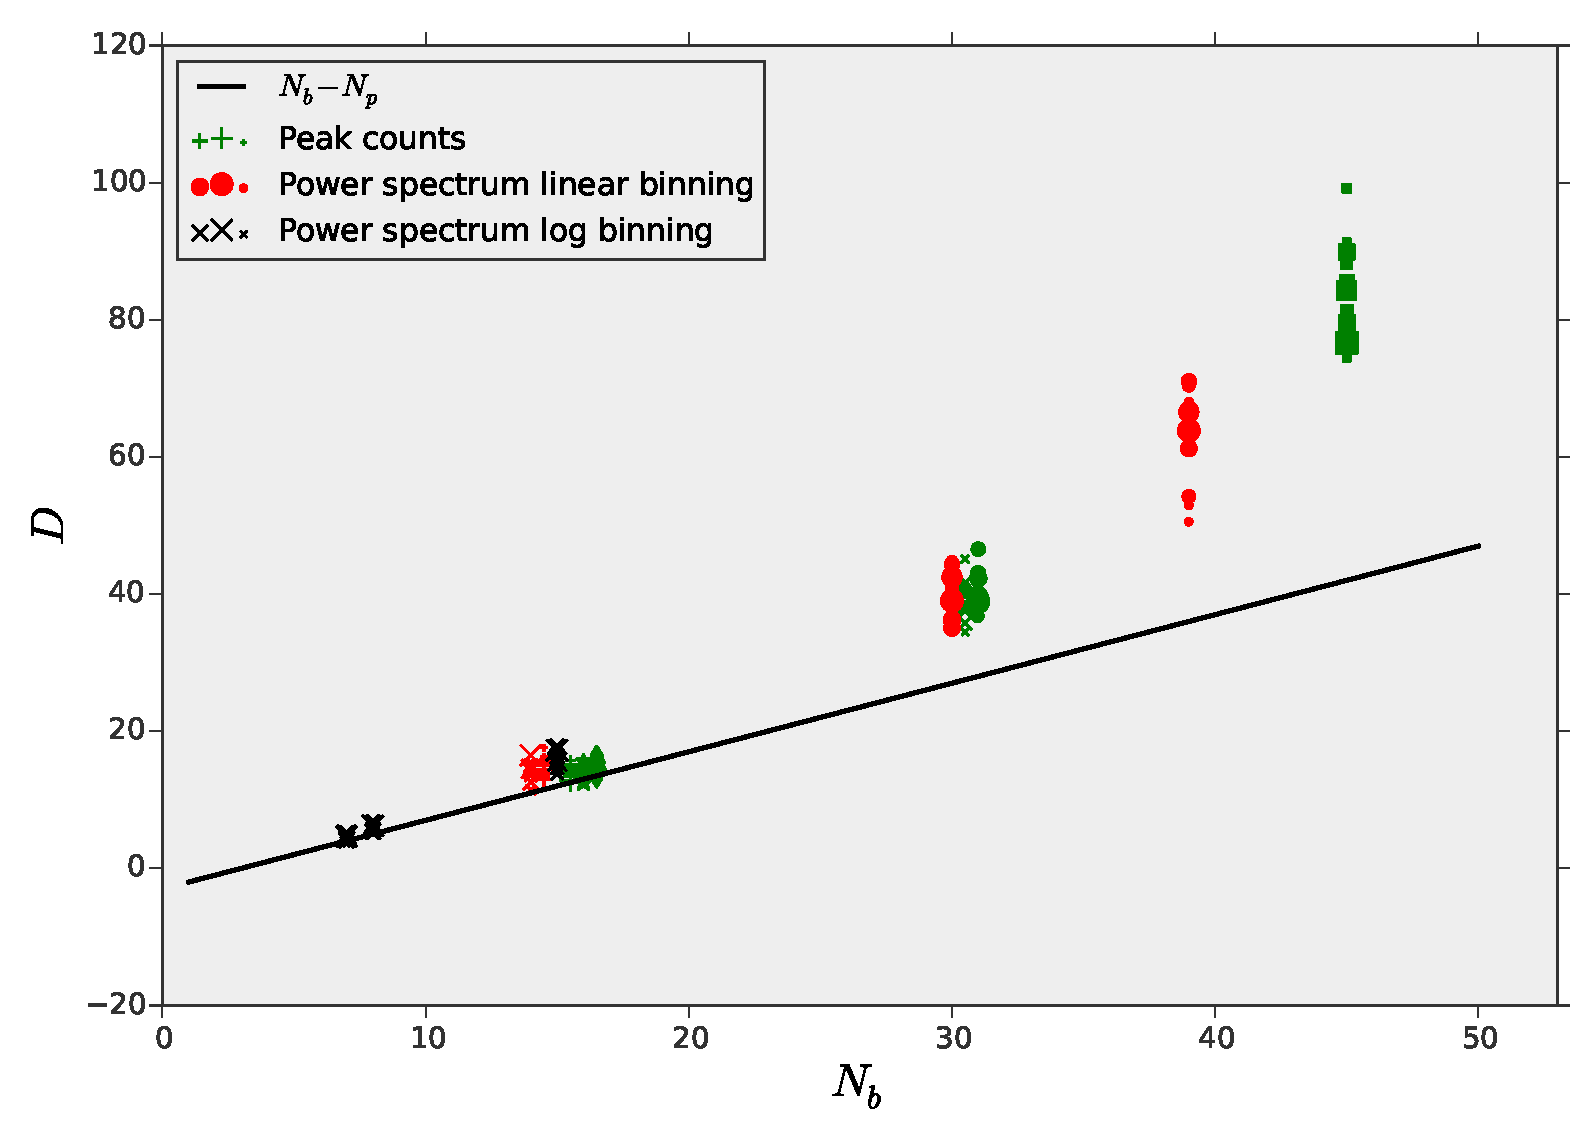
\includegraphics[scale=0.3]{Figures/effective_nb.eps}
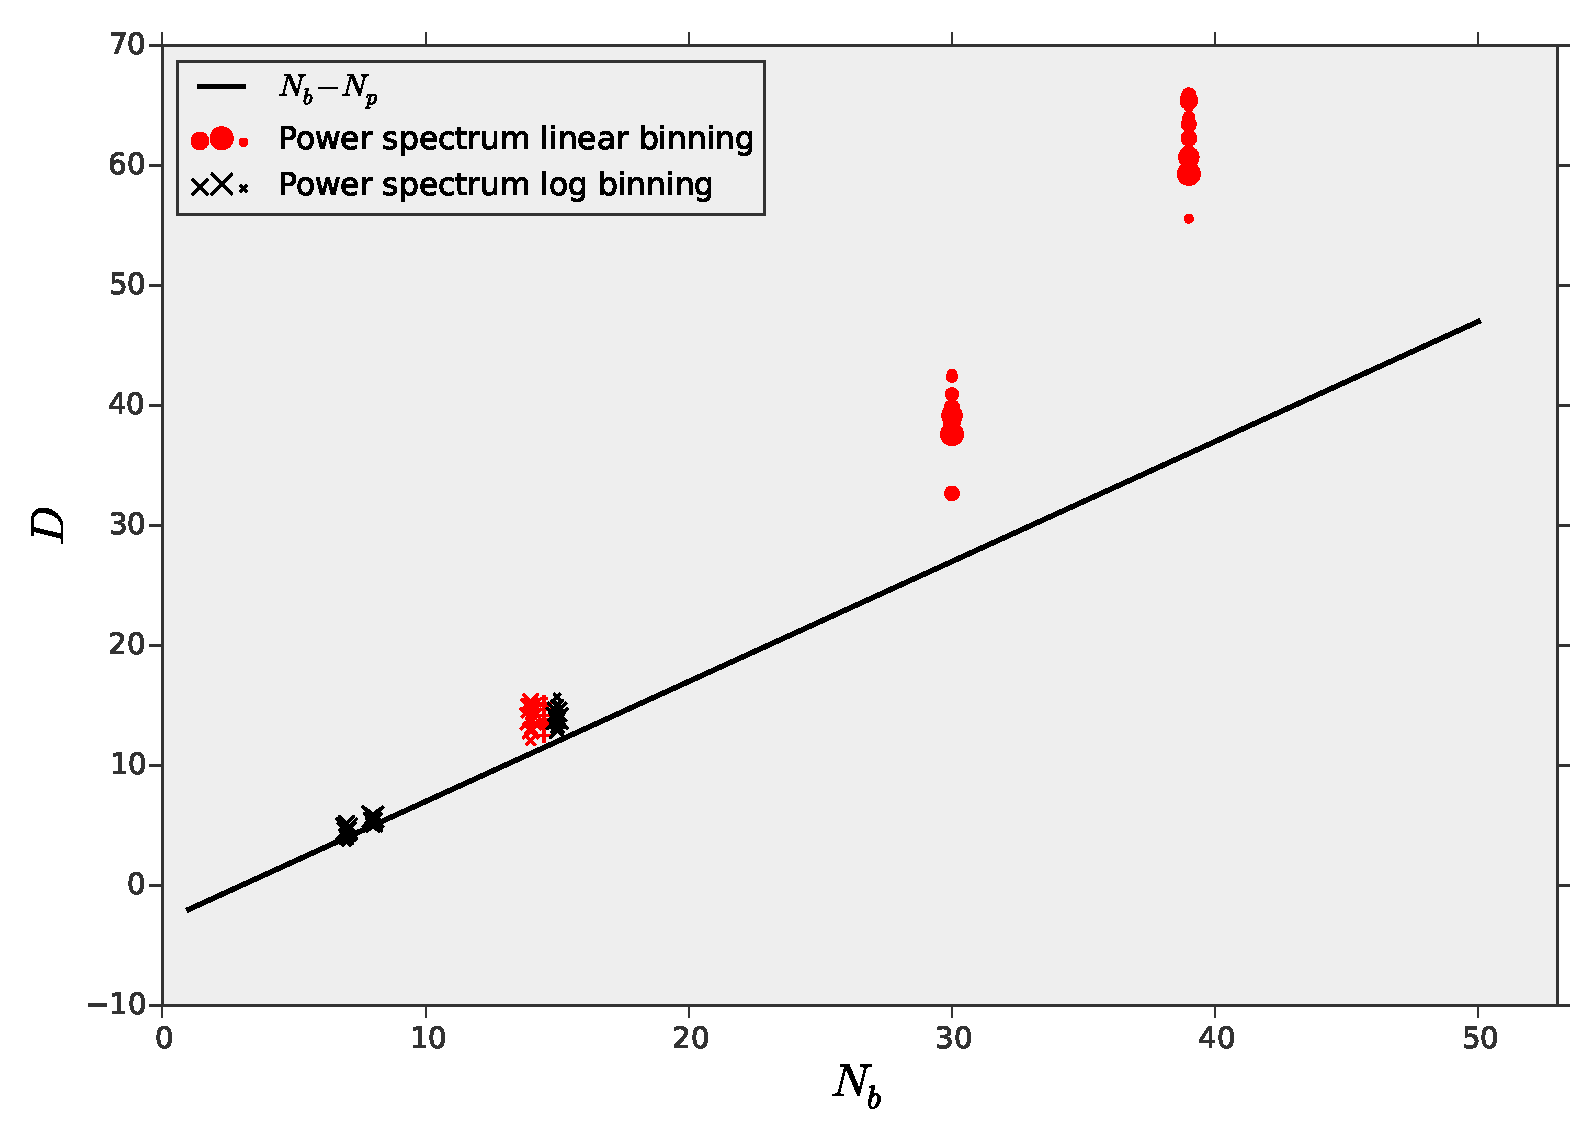
\includegraphics[scale=0.3]{Figures/effective_nb_gaussian.eps}
\caption{Effective dimesionality of the feature space, $D$, as a function of the number of bands $N_b$, for the features outlined in Table \ref{featuretable}.}
\label{effectivenb}
\end{figure*}

%%%%%%%%%%%%%%%%%%%%%%%%%%%%%%%%%%%%%%%%%%%%%%%%%%%%%%%%%%%%%%%%%%%%%%

\subsection{Parameter inference}
%
Let $\bbh{d}$ be the measured feature of dimension $N_b$, $\bb{d}(\bb{p})$ be the simulated feature at a point $\bb{p}$ in parameter space (which has a dimension $N_p$) and $\bb{C}$ be the $N_b\times N_b$ feature covariance matrix. For the purpose of this work $\bb{p}$ is the triplet $(\Omega_m,w,\sigma_8)$ and $\bb{d}$ is the convergence power spectrum $P^{\kappa\kappa}$, which is measured at $N_b=15$ log--spaced bands between $l\in[100,6000]$. While $d_M(\bb{p})$ can usually be predicted reasonably accurately by already existing emulators (see \citep{coyote2,Nicaea} for example), the matter is more complicated for covariance matrices. Measuring $\bb{C}$ from simulations involves generating a series of mock realizations $\bbh{d}_r$ with $r=1...N_r$ and estimating the sample covariance $\bbh{C}$

\begin{equation}
\bb{\bar{d}} = \frac{1}{N_r}\sum_{r=1}^{N_r} \bbh{d}_r
\end{equation}

\begin{equation}
\label{covest}
\bbh{C} = \frac{1}{N_r-1}\sum_{r=1}^{N_r} (\bbh{d}_r - \bar{\bb{d}}) (\bbh{d}_r - \bar{\bb{d}})^T
\end{equation}
%
Assuming a normal feature likelihood, together with a flat prior on the parameter space, the parameter posterior distribution $\mathcal{L}(\bb{p}\vert\bbh{d})$ can be obtained using Bayes theorem
\begin{equation}
\label{posteriorbayes}
\mathcal{L}(\bb{p}\vert\bbh{d}) = \mathcal{N}_\mathcal{L}\exp{\left[-\frac{1}{2}(\bbh{d}-\bb{d}(\bb{p}))^T\bb{C}^{-1}(\bbh{d}-\bb{d}(\bb{p}))\right]}
\end{equation}
%
For the sake of simplicity, we approximate the posterior as a Gaussian around its maximum. This is easily done approximating the simulated feature at first order around a point $\bb{p}_0$ (that ideally is the maximum of (\ref{posteriorbayes}))
\begin{equation}
\bb{d}(\bb{p}) \approx \bb{d}_0 + \bb{d}_0^\prime(\bb{p}-\bb{p}_0) 
\end{equation}
%
To measure the feature derivatives $\bb{d}'_0$ with respect to cosmology, we make use of the public code code NICAEA \citep{Nicaea} for the power spectrum, and we use an independent simulation set (that contains mocks at different combinations of $(\Omega_m,w,\sigma_8)$) for the peak counts.
We can build the estimator for the posterior location parameter $\bbh{p}$, given the observation $\bbh{d}$, as follows:
%
\begin{equation}
\label{estimatormean}
\bbh{p} = \bb{p}_0 + \bbh{T}(\bbh{d}-\bb{d}_0)
\end{equation}

\begin{equation}
\bbh{T} = (\bb{d}_0'^T\bbh{C}^{-1}\bb{d}_0')^{-1}\bb{d}_0'^T\bbh{C}^{-1}
\end{equation}
%
Defining the \textit{precision matrix} $\bbh{\Psi}=\bbh{C}^{-1}$, we can express the estimator of the parameter covariance as 

\begin{equation}
\label{estimatorcovariance}
\h{\Sigma}_\bb{p} = \bbh{F}^{-1}\bb{d}_0'^T\bbh{\Psi}\bb{C}\bbh{\Psi}\bb{d}_0'\bbh{F}^{-1}
\end{equation}

\begin{equation}
\label{estimatorfisher}
\bbh{F} = \bb{d}_0'^T\bbh{\Psi}\bb{d}_0'
\end{equation}
%
Where we introduced the Fisher matrix estimator $\bbh{F} = \bb{d}_0'^T\bbh{\Psi}\bb{d}_0'$ and, for simplicity, we assumed $\langle\bbh{d}\rangle=\bb{d}_0$, so that $\langle(\bbh{d}-\bb{d}_0)(\bbh{d}-\bb{d}_0)^T\rangle=\bb{C}$. 
The noise in the covariance estimator (\ref{covest}) and its inverse $\bbh{\Psi}$ propagates all the way to the posterior (\ref{posteriorbayes}), the parameter estimate (\ref{estimatormean}) and its variance (\ref{estimatorcovariance}). Following \citep{Taylor12} we can say that, if the feature vector $\bbh{d}$ from which $\bbh{C}$ is estimated is drawn from a multivariate Gaussian distribution, the precision matrix estimator $\bbh{\Psi}$ is biased
\begin{equation}
\label{psibias}
\langle\bbh{\Psi}\rangle = \frac{N_r-1}{N_r-N_b-2}\bb{\Psi}
\end{equation}
%
and, once the bias is corrected, the residual fluctuations in $\bbh{\Psi}$ are correlated as follows
\begin{equation}
\label{psifluctuations}
\langle\delta\h{\Psi}_{ij}\delta\h{\Psi}_{kl}\rangle = A\Psi_{ij}\Psi_{kl} + B(\Psi_{ik}\Psi_{jl} + \Psi_{il}\Psi_{jk})
\end{equation}
%
where $A,B$ are constants that depend on $N_r,N_b$ and have the asymptotic behavior $A\propto1/N_r^2,B\propto1/N_r$. We want to estimate the effect of these fluctuations on the parameter constraints $\Sigma_\bb{p}$, following the guidelines of \citep{DodelsonSchneider13}. We consider three cases:
\begin{itemize}
\item If the true data covariance $\bb{C}$ is known, the estimator (\ref{estimatorcovariance}) is biased, and the dominant contribution of the bias comes from the second order fluctuations in $\bbh{\Psi}$. Once the expectation values are taken as in (\ref{psifluctuations}), the bias sums up to 

\begin{equation}
\label{dodelsonscaling}
\langle\h{\Sigma}_\bb{p}\rangle=\Sigma_\bb{p}(1+B(N_b-N_p))
\end{equation}
%
This is the result obtained by \citep{DodelsonSchneider13}.

\item If we are not interested in measuring the location parameter $\bbh{p}$, but just the width of the parameter posterior, we are tempted to estimate errorbars purely from simulations, replacing the true covariance $\bb{C}$ with its estimator $\bbh{C}$, measured from the same simulation set we use to compute $\bbh{\Psi}$. If we do that, and we do not correct for the bias (\ref{psibias}), the parameter variance will have a contribution from both the second and first order fluctuations in $\bbh{\Psi}$, which now have a non zero expectation value. In this case the bias sums up to 
\begin{equation}
\label{mockscalinguncorrected}
\langle\h{\Sigma}_\bb{p}\rangle=\Sigma_\bb{p}(1-(1+N_b)/N_r+B(1+N_p))
\end{equation}

\item If we repeat the same exercise as above, but we correct for the bias in the precision matrix estimator, we are left with 

\begin{equation}
\label{mockscalingcorrected}
\langle\h{\Sigma}_\bb{p}\rangle=\Sigma_\bb{p}(1+B(1+N_p))
\end{equation}

\end{itemize} 
%
The complete calculations that justify (\ref{dodelsonscaling}),(\ref{mockscalinguncorrected}) and (\ref{mockscalingcorrected}) are shown in the Appendix. The last two examples have to be considered as academic exercises, as in a real experiment the data $\bbh{d}$ and its covariance matrix regulate the scatter of the $\bbh{p}$ estimator. With the $\bbh{d}$ Gaussianity assumption, the coefficient $B$ can be calculated exactly as \citep{DodelsonSchneider13,Taylor12}, and tends to $1/N_r$ in the limit of $N_r\gg N_b$. This leads to a degradation of order $D/N_r$ for the variance of each estimated parameter $\sigma^2_p=\Sigma_{pp}$. We test the scaling relation
\begin{equation}
\label{ourscaling}
\langle\h{\sigma}_p^2\rangle = \sigma^2_p(N_s)\left(1+\frac{D}{N_r}\right)
\end{equation}
%
on our simulations. We call $D$ the \textit{effective dimensionality} of the feature space which, under Gaussianity assumptions, is equal to $D=N_b-N_p$ in the case where the true covariance $\bb{C}$ is known, $D=N_p-N_b$ when the true data covariance is replaced by its estimator (computed from the same simulation set) but the biased $\bbh{\Psi}$ estimator is used, and $D=1+N_p$ when the $\bbh{\Psi}$ bias is corrected. 

We compute the expectation values of $\h{\sigma}^2_p$ (equations (\ref{estimatorcovariance}),(\ref{ourscaling})) averaging over 100 random resamplings of our shear ensembles. For the true feature covariance matrix $\langle(\bbh{d}-\bb{d}_0)(\bbh{d}-\bb{d}_0)^T\rangle=\bb{C}$ we use the estimated covariance from a grand ensemble built with the union of all the ensembles with different $N_s$. 

The true parameter variance $\sigma^2_p(N_s)$ in principle depends on the number of independent $N$--body simulations $N_s$, which appears in the randomization procedure we describe in \S~\ref{shearsim}. The reason for this can be found in that, if $N_s$ is not big enough, the different shear realizations cannot be all independent, and hence the true variance $\sigma^2_p(N_s\rightarrow\infty)$ cannot be recovered in the limit $N_r\rightarrow\infty$. In particular there could be some residual error in the expectation value of (\ref{estimatorcovariance}) even if $N_r$ is big. In the next paragraph we outline our main findings.
 

%%%%%%%%%%%%%%%%%%% RESULTS %%%%%%%%%%%%%%%%%%%%%%%%%%%%%%%%%%%%%%%

\section{Results} 

In this section we outline the main results of this work. We show the qualitative behavior of the $P^{\kappa\kappa}$ probability distribution function (PDF) in ensembles built with different $N_s$. We also show how the forecasts on the Dark Energy equation of state, $w$, depend on $N_s$ and $N_r$. Figure \ref{ps_pdf} shows the power spectrum PDF at four selected multipoles, while Figure \ref{ps_var} shows the variance in each multipole. This result is compared to the one that we would obtain assuming that the convergence is a Gaussian random field
\begin{equation}
\label{gaussianvar}
\mathrm{Var}(P^{\kappa\kappa}(l)) = \frac{P^{\kappa\kappa,2}(l)}{N(l)}
\end{equation}
%
where $N(l)$ is the number of modes used to estimate the power spectrum at $l$. $N_l$ is measured from the Fourier trasformed image grid. Figure \ref{wvar_nr} show the scaling of the expectation value of $\h{\sigma}_w^2$ with the number of mocks $N_r$ using the power spectrum and compare it with the known result obtained in \citep{DodelsonSchneider13} and expressed in equation (\ref{ourscaling}). Figure \ref{wvar_ns} shows the effect of varying $N_s$ on the $w$ constraint. Finally Figure \ref{effectivenb} shows how the effective feature dimensionality $D$ depends on the number of bands $N_b$, for a variety of features and binning choices outlined in Table \ref{featuretable}. 

%%%%%%%%%%%%%%%%%% DISCUSSION %%%%%%%%%%%%%%%%%%%%%%%%%%%%%%%%%%%%%

\section{Discussion}

In this section we discuss our main findings. Figure \ref{ps_pdf} shows that, although different choices of $N_s$ do not seem to affect the power spectrum PDF at large scales (top two panels), there are some qualitative differences on small scales (bottom two panels), on which a shear ensemble built with a small $N_s$ does not have the same statistical behavior of ensembles built with large $N_s$. Looking at the black curves, we see that the $N_s=1$ ensembles exibit some stochastic fluctuations in where the PDF peaks. We need as small as $N_s=2$ to recover the right location parameter for the power spectrum on small scales. 

Figure \ref{ps_var} shows the variance of convergence power spectrum computed from different ensembles, in units of the Gaussian expectation. We find that, even with $N_s=1$, our results are in good agreement with the ones obtained by \citep{Sato12}, which used $N_s=400$. This fact by itself is not sufficient to conclude that $N_s$ does not have an effect on parameter inferences, since these depend on the cross band covariances. 

In Figure \ref{wvar_nr} we examine how the $w$ constraint depends on the number of mocks used to estimate the covariance, and we find good agreement with (\ref{ourscaling}). In particular we can see that one $N$--body simulation is enough to construct an ensemble of $O(10^5)$ mutually independent mock power spectra, for which the $w$ constraint scales like $1/N_r$ all the way to $N_r=10^5$.    

Figure \ref{wvar_ns} shows the dependence of the dark energy constraint with $N_s$. We find that, in the range $N_s\in[1,200]$ the $w$ inferred variance $\sigma_0^2$ fluctuates stochastically and does not show an appreciable trend with $N_s$. 

We determine the effective dimensionality of the feature space, $D$, with a linear regression using equation (\ref{ourscaling}), for the set of features outlined in Table \ref{featuretable}. The results shown in Figure \ref{effectivenb}, however, show that the feature dimensionality $D$ grows faster than the linear $O(N_b)$ optimistic case predicted by \citep{DodelsonSchneider13}. When we estimate the real data covariance $\bb{C}$ from the same simulation set used to measure $\bbh{C}$, the effective dimensionality $D$ shows the expected behavior. More in detail, the toy models (\ref{mockscalinguncorrected}) and (\ref{mockscalingcorrected}) tell us that when we do not correct for the bias in the $\bbh{\Psi}$ estimator the effective dimensionality is negative (assuming $N_b>N_p$) and the parameter variance is underestimated when $N_r$ is not large enough. This explains what \citep{MinkPetri} observe in their Figures 7,8.  

%%%%%%%%%%%%%%%%%% CONCLUSION %%%%%%%%%%%%%%%%%%%%%%%%%%%%%%%%%%%%%

\section{Conclusion}

In this work we examine the effect of $N$--body simulations based shear ensembles on forecasted cosmological constraints. Our main results can be summarized as follows:

\begin{itemize}
\item We can recycle a single $N$--body simulation to produce an ensemble of $O(10^5)$ independent maps. The mean feature measured from a shear ensemble, though, could be inaccurate if only one $N$--body simulation is used.  
\item The $1/N_r$ scaling for the dark energy constraint has been verified in our simulations, but the effective dimensionality $D$, that regulates the degradation of the error bars, grows faster than the $O(N_b)$ that \citep{DodelsonSchneider13} predicted. 
\item The fluctuations in the $w$ forecasted variance do not exibit an appreciable trend with $N_s$ 
\end{itemize}
%
Future prospects of this work involve extending this analysis to more general feature spaces, such as the ones that characterize non--Gaussian statistics such as shear peaks and higher moments of $\kappa$ fields. In order to scale these considerations to future surveys such as LSST, it is necessary to see if our findinds hold when challenged by larger and higher resolutions $N$--body simulations.  

%%%%%%%%%%%%%%%%%%%%%%%%%% ACKNOWLEDGMENTS %%%%%%%%%%%%%%%%%%%%%%%%%%%%%%%%%%%%%%%%%%%%%%%%%%%%%%
 

\section*{Acknowledgements}

\bibliography{ref}

%%%%%%%%%%%%%%%%%%%%%%%%%% APPENDIX %%%%%%%%%%%%%%%%%%%%%%%%%%%%%%%%%%%%%%%%%%%%%%%%%%%%%%

\section*{Appendix: scaling of the effective dimensionality}
\label{appendix}

The goal of this appendix is giving a derivation of (\ref{dodelsonscaling}),(\ref{mockscalinguncorrected}) and (\ref{mockscalingcorrected}) following the guidelines from \citep{DodelsonSchneider13,Taylor12}. First consider the case in which we use the same simulation set to estimate $\bb{C},\bbh{\Psi}$: in this case equation (\ref{estimatorcovariance}) reduces to the inverse Fisher estimator $\h{\Sigma}_\bb{p}=\bbh{F}^{-1}$. If we write $\bbh{F}=\bb{F}+\delta\bbh{F}=\bb{F}+\bb{d}_0'^T\delta\bbh{\Psi}\bb{d}_0'$, and expand at second order in the fluctuations we get

\begin{equation}
\h{\Sigma}_\bb{p} = \bb{F}^{-1} + \bb{F}^{-1}\left(- \delta{\bbh{F}}+ \delta{\bbh{F}}\bb{F}^{-1}\delta{\bbh{F}}\right)\bb{F}^{-1}  
\end{equation}  
%
If we use the precision estimator $\bbh{\Psi}=\bb{\Psi}+\delta\bbh{\Psi}$ and do not correct for the bias (\ref{psibias}), we have to use the facts that
\begin{equation}
\begin{matrix}
& \langle\delta\bbh{\Psi}\rangle = \frac{1+N_b}{N_r-N_b-2}\bb{\Psi} \\ \\
& \langle\delta\h{\Psi}_{ij}\delta\h{\Psi}_{kl}\rangle = \frac{A([(N_r-1)^2+(1+N_b)^2]\Psi_{ij}\Psi_{kl} + B(N_r-1)^2(\Psi_{ik}\Psi_{kl}+\Psi_{il}\Psi_{jk})}{(N_r-N_b-2)^2}
\end{matrix}
\end{equation}
%
Keeping only the leading order $O(1/N_r)$ in the expansion we get the results
\begin{equation}
\label{explanationuncorrected}
\begin{matrix}
& \langle\delta\bbh{F}\rangle = \left(\frac{1+N_b}{N_r}\right)\bb{F} \\ \\
& \langle\delta{\bbh{F}}\bb{F}^{-1}\delta{\bbh{F}}\rangle = B(1+N_p)\bb{F}
\end{matrix}
\end{equation}
%
which leads immediately to (\ref{mockscalinguncorrected}). Now suppose we correct for the bias in the precision estimator, and use the unbiased $\bbh{\Psi}$ for which $\delta\bbh{\Psi}=0$. This leads to equation (\ref{psifluctuations}) for the quadratic fluctuations in the precision matrix, and to the same (\ref{explanationuncorrected}), except for $\langle\delta\bbh{F}\rangle=0$. This leads to (\ref{mockscalingcorrected}). If now we keep $\bb{C}$ fixed and we estimate only $\bbh{\Psi}$ from the simulations, we get
\begin{equation}
\label{tempcovarianceestimate}
\h{\Sigma}_\bb{p} = (\bbh{F}+\delta\bbh{F})^{-1}\bb{d}_0'^T(\bbh{\Psi}+\delta\bbh{\Psi})\bb{C}(\bbh{\Psi}+\delta\bbh{\Psi})\bb{d}_0'(\bbh{F}+\delta\bbh{F})^{-1}
\end{equation}
%
If we isolate the second order terms in (\ref{tempcovarianceestimate}), the result is 
\begin{equation}
\h{\Sigma}_\bb{p}\vert_2 = \bb{F}^{-1}(\bb{d}_0'^T\delta\bbh{\Psi}\bb{C}\delta\bbh{\Psi}\bb{d}_0'-\delta{\bbh{F}}\bb{F}^{-1}\delta{\bbh{F}})\bb{F}^{-1}
\end{equation} 
%
The expectation values of the quadratic fluctuations are easily computed using (\ref{psifluctuations}):
\begin{equation}
\begin{matrix}
& \langle\bb{d}_0'^T\delta\bbh{\Psi}\bb{C}\delta\bbh{\Psi}\bb{d}_0'\rangle = B(1+N_b)\bb{F} \\ \\
& \langle\delta{\bbh{F}}\bb{F}^{-1}\delta{\bbh{F}}\rangle = B(1+N_p)\bb{F}
\end{matrix}
\end{equation}
%
From which (\ref{dodelsonscaling}) immediately follows. 
\label{lastpage}
\end{document}
